% vim:encoding=utf8 ft=tex sts=2 sw=2 et:

\documentclass{classrep}
\usepackage[utf8]{inputenc}
\usepackage{natbib} % potrzba do bibliografii
\usepackage{listings}
\usepackage{graphicx}
\usepackage{amsmath}
\usepackage{amsfonts}
\usepackage{amssymb}
\usepackage{amsthm}
\usepackage{polski}
\usepackage[hidelinks]{hyperref}
\usepackage{lmodern}  % for bold teletype font
\usepackage{amsmath}  % for \hookrightarrow
\usepackage{xcolor}   % for \textcolor
\usepackage{listings}
\usepackage{lipsum}
\usepackage{longtable}

\lstset{
  basicstyle=\ttfamily,
  columns=fullflexible,
  frame=single,
  breaklines=true,
  postbreak=\mbox{\textcolor{red}{$\hookrightarrow$}\space},
}


\newtheorem{definition}{Definicja}
\newtheorem{theorem}{Twierdzenie}

\studycycle{Informatyka, studia zaoczne, inż I st.}
\coursesemester{V}

%\coursename{Angelologia teoretyczna i stosowana}
\coursename{Sztuczna inteligencja i systemy ekspertowe}
\courseyear{2017/2018}

\courseteacher{mgr inż. Paweł Tarasiuk}
\coursegroup{sobota, 14:45}

\author{
  \studentinfo{Natalia Mateuszuk}{203940} \and
  \studentinfo{Adrian Grzelak}{200242}
}

\title{Zadanie 1 \\
Przeszukiwanie przestrzeni stanów. Piętnastka}
%\svnurl{http://serce.ics.p.lodz.pl/svn/labs/atis/b_wt1415/grupa/zad1@134}

\begin{document}
\maketitle

\section{Wstęp}
Piętnastka to popularna łamigłówka polegająca na przesuwaniu wolnego pola po planszy o rozmiarze $3 \times 3$ aż do momentu ułożenia całej układanki. W raporcie tym zostaną przedstawione odpowiedzi na kilka ciekawych pytań dotyczących tej łamigłówki, oraz analiza skuteczności algorytmów przeszukiwań drzew, na podstawie poszukiwania rozwiązania właśnie tej piętnastki. Ponadto przeanalizujemy jej pochodne, czyli plansze o rozmiarach niestandardowych jak np. $3 \times 3$, $2 \times 2$, $3 \times 2$ itp.

\begin{center}
	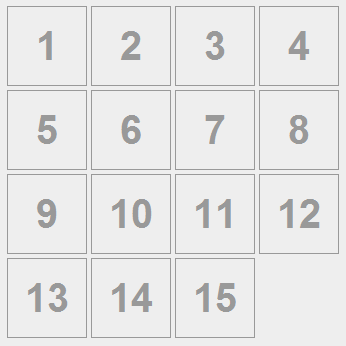
\includegraphics[height=6cm]{puzzle.png}
	
	\textbf{Rysunek} Ułożona tablica piętnastka
\end{center}

\section{Analiza rozwiązania}
\subsection{Czy zawsze można rozwiązać?}
Nie. Łatwo można się o tym przekonać na tej tablicy $2 \times 2$, nie ważne co zrobimy nie uda nam się zamienić miejscami klocków 2 i 3 bez zmiany pozycji klocka nr 1.
\begin{center}
	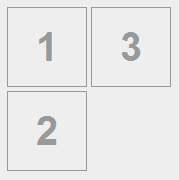
\includegraphics[height=3cm]{2x2unsolvable.png}
	
	\textbf{Rysunek} Nierozwiązywalna plansza
\end{center}

Każdą układankę o 1 wierszu lub 1 kolumnie da się ułożyć tylko wtedy gdy liczby są posortowane rosnąco. Co w przypadku tablicy $n\times m$ gdzie $n,m\geqslant2$ ? W swojej pracy \textit{Analysis of the Sixteen Puzzle}\citep{sixteen} Kevin Gong udowadnia że początkowy układ możemy stosunkowo łatwo sprawdzić pod względem rozwiązywalności. W tym celu zdefiniujemy \textbf{liczbę inwersji} dla uporządkowanego ciągu liczb.
\begin{definition}
Uporządkowany zbiór $A=(x_1,x_2,...,x_n)$ posiada k-inwersji jeżeli $x_i < x_j$ w przypadku gdy $i > j$ dla k różnych par $i$,$j$.
\end{definition}

Przykładowo, permutacja $(1, 2, 4, 3)$ ma jedną inwersję $4 > 3$. Permutacja $(3, 1, 2, 4)$ ma dwie inwersje $3 > 1$, $3 > 2$. $(1, 2, 3, 4)$ nie ma żadnych.

Dla układanek o rozmiarach $n\times m$ gdzie $n,m\geqslant2$ prawdziwe są następujące twierdzenia:
\begin{theorem}\label{pierwsze}
\citep{sixteen} Jeżeli liczba kolumn w układance jest nieparzysta, to każda poprawna konfiguracja   odpowiada permutacji z parzystą liczbą inwersji.
\end{theorem}
\begin{theorem}
\citep{sixteen} Jeżeli liczba kolumn w układance jest parzysta, to każda poprawna konfiguracja   która posiada pusty element w $i$-tym wierszu, a liczba wierszy pomniejszona o $i$ ($m-i$),jest liczbą parzystą - posiada parzystą liczbą inwersji.
\end{theorem}
\begin{theorem}\label{trzecie}
\citep{sixteen} Jeżeli liczba kolumn w układance jest parzysta, to każda poprawna konfiguracja   która posiada pusty element w $i$-tym wierszu, a liczba wierszy pomniejszona o $i$ ($m-i$),jest liczbą nieparzystą - posiada nieparzystą liczbą inwersji.
\end{theorem}
Sprawdźmy zatem poniższą tablicę przy pomocy powyższych twierdzeń
\begin{center}
	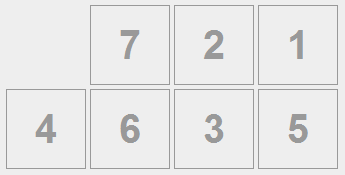
\includegraphics[height=3cm]{2x4unsolvable.png}
	
	\textbf{Rysunek} Plansza 2x4
\end{center}
Odpowiadająca jej permutacja to $(7, 2, 1, 4, 6, 3, 5)$. Liczba kolumn jest parzysta, zatem nie skorzystamy z Twierdzenia \ref{pierwsze}. Liczba wierszy pomniejszona indeks wiersza w którym znajduje się element pusty (m-i) jest równa 1 czyli jest liczbą nieparzystą (Twierdzenie \ref{trzecie}). W takim przypadku oczekujemy że liczba inwersji również będzie nieparzysta, aby układanka dała się rozwiązać. Niestety $6 + 1 + 1 + 2 = 10$ zatem układanka ta nie da się rozwiązać.

Powyższe twierdzenia przekładają się na następujący algorytm sprawdzający:
\lstinputlisting[language=C,breaklines=true]{board_is_sorted.cpp}

\subsection{Ilość dostępnych permutacji tablicy}

\begin{theorem}
\citep{sixteen} W przypadku tablicy o jednej kolumnie lub jednym wierszu, oczywistym jest że liczba możliwych stanów jest równa liczbie wszystkich elementów tablicy. W przypadku gdy tablica ma rozmiar $n\times m$ gdzie $n,m>1$ Istnieje dokładnie $\frac{(n\times m)!}{2}$ rozwiązywalnych konfiguracji. 
\end{theorem}

Poniższa tabela podaje nam liczbe rozwiązywalnych stanów w poszczególnych rozmiarach układanki.
\begin{center}
\begin{longtable}{|r|r|}
  \hline 
  Rozmiar Tablicy & Rozwiązywalne stany\\
  \hline
    $1 \times n$ & n \\
  \hline
  	$2 \times 2$ & 12 \\
  \hline
    $2 \times 3$ & 360 \\
  \hline
    $2 \times 4$ & 20 160 \\
  \hline
    $2 \times 5$ & 1 814 400 \\
  \hline
    $2 \times 6$ & 239 500 800 \\
  \hline
    $2 \times 7$ & 43 589 145 600 \\
  \hline
    $2 \times 8$ & 10 461 394 944 000 \\
  \hline
    $3 \times 3$ & 181 440 \\
  \hline
    $3 \times 4$ & 239 500 800 \\
  \hline
    $3 \times 5$ & 653 837 184 000 \\
  \hline
    $4 \times 4$ & 10 461 394 944 000 \\
  \hline
\end{longtable} 

\textbf{Tabela.} Liczba możliwych stanów w zależności od rozmiaru
\end{center}
Oczywiście tabela rozszerza się na większe rozmiary, jednakże w naszym programie ze względu na ograniczenia pamięci i sprzętowe, rozpatrujemy tablice o maksymalnie 16 elementach.

Warto wspomnieć że w przypadku losowania tablicy do dalszej części eksperymentu, około połowa przypadków była nierozwiązywalna. Wynika to z faktu, że istnieje dokładnie tyle samo stanów nierozwiązywalnych co rozwiązywalnych. Dowiedzione to zostało w pracy \citep{sixteen}\textit{Analysis of the Sixteen Puzzle}.

\section{Algorytm BFS}
Algorytm przeszukiwania grafu wszerz polega na pobieraniu najpierw najbliższych sąsiadów w grafie , sprawdzanie ich stanów i dopiero potem pobierania "poziom niżej". Tak zdefiniowany sposób zawsze znajdzie nam najkrótszą drogę, jednakże musi wykonać bardzo dużą liczbę porównań. Poniżej w tabeli przedstawione są wyniki z kilkunastu prób algorytmu BFS z losowego stanu początkowego.
\begin{center}
\begin{longtable}{|r|r|r|r|}
  \hline 
  Rozmiar Tablicy & Długość Ścieżki & Odwiedzone stany & Czas rozwiązania \\
  	\hline
		$2 \times 2$ & 5 & 10 & 0ms \\
	\hline
		$2 \times 2$ & 6 & 12 & 0ms \\
	\hline
		$2 \times 2$ & 6 & 12 & 0ms \\
	\hline
		$3 \times 2$ & 14 & 219 & 0ms \\
	\hline
		$3 \times 2$ & 14 & 215 & 0ms \\
	\hline
		$2 \times 3$ & 9 & 61 & 0ms \\
	\hline
		$2 \times 3$ & 13 & 157 & 0ms \\
	\hline
		$2 \times 4$ & 23 & 8 707 & 12ms \\
	\hline
		$2 \times 4$ & 19 & 4 906 & 6ms \\
	\hline
		$2 \times 4$ & 25 & 13 776 & 20ms \\
	\hline
		$3 \times 3$ & 24 & 119 896 & 269ms \\
	\hline
		$3 \times 3$ & 22 & 92 739 & 150ms \\
	\hline
		$3 \times 3$ & 18 & 20 101 & 24ms \\
	\hline
		$3 \times 3$ & 20 & 54 782 & 73ms \\
	\hline
		$3 \times 3$ & 18 & 19 819 & 34ms \\
	\hline
		$3 \times 3$ & 24 & 116 132 & 202ms \\
	\hline
		$3 \times 3$ & 26 & 158 738 & 314ms \\
	\hline
		$3 \times 3$ & 23 & 103 843 & 171ms \\
	\hline
		$3 \times 3$ & 25 & 155 378 & 291ms \\
	\hline
		$2 \times 6$ & Nie osiągnięto & 48 814 626 & $\sim 75$s \\
	\hline
		$2 \times 6$ & Nie osiągnięto & 48 814 626 & $\sim 75$s \\
	\hline
		$2 \times 6$ & Nie osiągnięto & 48 665 982 & $\sim 75$s \\
	\hline
		$4 \times 4$ & Nie osiągnięto & 43 740 510 & $\sim 75$s \\
	\hline
		$4 \times 4$ & Nie osiągnięto & 43 749 238 & $\sim 75$s \\
	\hline
		$4 \times 4$ & Nie osiągnięto & 43 747 957 & $\sim 75$s \\
	\hline
		$4 \times 4$ & Nie osiągnięto & 43 746 019 & $\sim 75$s \\

	\hline
\end{longtable} 
\textbf{Tabela.} Wyniki dla algorytmu BFS.
\end{center}
Jak widzimy w przypadku tego algorytmu (Możemy to głównie zaobserwować z przypadków $3 \times 3$) algorytm zwykle odnajduje ścieżkę po przejrzeniu znacznej ilości dostępnych stanów. Można wywnioskować że pomimo bardzo atrakcyjnych długości ścieżek (najkrótszych możliwych) algorytm jest mało wydajny.
 
\section{Algorytm DFS}
Algorytm przeszukiwania grafu w głąb przeszukuje w sposób analogiczny do algorytmu BFS, z tą różnicą że zamiast przejrzeć najpierw cały poziom, to przegląda najpierw całą ścieżkę. Dopiero gdy ta mu się kończy, to wraca do ostatniego rozgałęzienia i od kolejnej krawędzi rozpoczyna poszukiwanie znowu.
Tak zdefiniowany sposób znajduje niejednokrotnie ekstremalnie długie ścieżki. Poniżej w tabeli przedstawione są wyniki z kilkunastu prób algorytmu DFS z losowego stanu początkowego.
\begin{center}
\begin{longtable}{|r|r|r|r|}
  \hline 
  Rozmiar Tablicy & Długość Ścieżki & Odwiedzone stany & Czas rozwiązania \\
	\hline
		$2 \times 2$ & 2 & 3 & 0ms \\
	\hline
		$2 \times 2$ & 9 & 10 & 0ms \\
	\hline
		$2 \times 2$ & 9 & 10 & 0ms \\
	\hline
		$2 \times 3$ & 1 & 360 & 0ms \\
	\hline
		$2 \times 3$ & 120 & 161 & 0ms \\
	\hline
		$3 \times 2$ & 138 & 307 & 0ms \\
	\hline
		$4 \times 2$ & 2667 & 2 979 & 11ms \\
	\hline
		$4 \times 2$ & 8242 & 13 911 & 37ms \\
	\hline
		$4 \times 2$ & 5290 & 6 016 & 13ms \\
	\hline
		$3 \times 3$ & 54051 & 130 784 & 303ms \\
	\hline
		$3 \times 3$ & 59936 & 72 816 & 231ms \\
	\hline
		$3 \times 3$ & 19510 & 20 438 & 52ms \\
	\hline
		$3 \times 3$ & 56646 & 126 239 & 309ms \\
	\hline
		$3 \times 3$ & 38910 & 148 557 & 367ms \\
	\hline
		$3 \times 4$ & Nie osiągnięto & 23 841 458 & $\sim 75$s \\
	\hline
		$2 \times 6$ & Nie osiągnięto & 28 334 635 & $\sim 75$s \\
	\hline
		$2 \times 6$ & Nie osiągnięto & 28 334 887 & $\sim 75$s \\
	\hline
		$4 \times 4$ & Nie osiągnięto & 22 492 606 & $\sim 75$s \\
	\hline
		$4 \times 4$ & Nie osiągnięto & 22 493 316 & $\sim 75$s \\
	\hline
\end{longtable} 
\textbf{Tabela.} Wyniki dla algorytmu DFS.
\end{center}
Podobnie jak algorytm BFS algorytm ten również przegląda znaczną liczbę stanów przed odnalezieniem rozwiązania. W dodatku ścieżki otrzymane w jego wyniku są bardzo długie. W kontekście rozwiązywania piętnastki, trudno dostrzec zalety tego algorytmu w porównaniu do innych. Algorytm sprawdzi się lepiej tylko w bardzo szczególnych przypadkach.

\section{Algorytm A*}
Algorytm A* w celu usprawnienia przeszukiwania przyjmuje funkcję heurystyczną. Funkcja ta definiuje jakąś miarę podobieństwa między elementem odwiedzanym a poszukiwanym. W każdym kolejnym kroku wybieramy element który jest najbardziej podobny do poszukiwanego rozwiązania. Algorytmy A* mają znaczną przewagę nad BFS i DFS jeżeli tylko taką miarę da się zdefiniować i elementy podobne są blisko siebie.

\subsection{Heurestyka Tile On Place}
Heurystyka Tile On Place daje 1 punkt za to że element przebywa na swoim miejscu. Policzmy heurystykę dla poniższej tablicy.
\begin{center}
	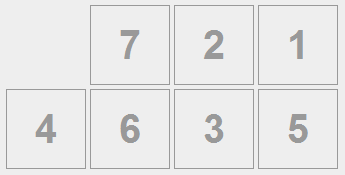
\includegraphics[height=3cm]{2x4unsolvable.png}
\end{center}
Jak widzimy jedynie element "6" jest na właściwym miejscu. Zatem funkcja zwróci nam wartość 1. Do dalszego przeszukiwania wybierane są elementy ze zmaksymalizowaną wartością heurystyki. Poniżej w tabeli przedstawione są wyniki z kilkunastu prób algorytmu A* z heurystyką Tile on Place z losowego stanu początkowego.
\begin{center}
\begin{longtable}{|r|r|r|r|}
  \hline 
  Rozmiar Tablicy & Długość Ścieżki & Odwiedzone stany & Czas rozwiązania \\
	\hline
		$2 \times 2$ & 0 & 1 & 0ms \\
	\hline
		$2 \times 2$ & 2 & 3 & 0ms \\
	\hline
		$2 \times 2$ & 3 & 4 & 0ms \\
	\hline
		$2 \times 2$ & 8 & 9 & 0ms \\
	\hline
		$3 \times 3$ & 146 & 4 755 & 8ms \\
	\hline
		$3 \times 3$ & 57 & 297 & 0ms \\
	\hline
		$3 \times 4$ & 323 & 384 135 & 857ms \\
	\hline
		$3 \times 4$ & 189 & 21 642 & 43ms \\
	\hline
		$3 \times 4$ & 108 & 10 543 & 21ms \\
	\hline
		$3 \times 4$ & 298 & 384 058 & 997ms \\
	\hline
		$3 \times 4$ & 311 & 384 410 & 1105ms \\
	\hline
		$3 \times 4$ & 306 & 384 389 & 970ms \\
	\hline
		$4 \times 4$ & Nie Osiagnieto & 31 708 484 & $\sim 75$s \\
	\hline
		$4 \times 4$ & Nie Osiagnieto & 30 575 910 & $\sim 75$s \\
	\hline
\end{longtable} 
\textbf{Tabela.} Wyniki dla algorytmu A* z heurystyką Tile On Place.
\end{center}
To już są dużo lepsze pod względem liczby odwiedzonych stanów wyniki niż było to w przypadku algorytmów DFS i BFS. Ponadto udało nam się znaleźć rozwiązania układanek 3x4! (Wcześniejsze algorytmy nie znalazły, ze względu na ograniczenia sprzętowe) Z powodzeniem można stwierdzić że algorytmy wykorzystujące heurystykę do przeszukiwania przestrzeni stanów piętnastki zdecydowanie się nadają.
\subsection{Heurestyka Manhattan}
Heurystyka Manhattan daje każdej cyfrze na planszy liczbę punktów która odpowiada odległości w jakiej znajduje się od swojego miejsca w rozwiązaniu (Mówimy oczywiście o odległości w metryce Manhattan). Policzmy heurystykę dla poniższej tablicy. Poniżej w tabeli przedstawione są wyniki z kilkunastu prób algorytmu A* z heurystyką Manhattan z losowego stanu początkowego.
\begin{center}
	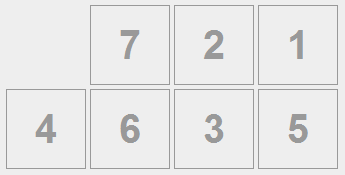
\includegraphics[height=3cm]{2x4unsolvable.png}
\end{center}
I tak kolejno policzmy dla każdej cyfry:
\begin{enumerate}
  \setcounter{enumi}{-1}
  \item (Puste Pole) Raz w dół i 3 razy w prawo. Zatem odległość 4.
  \item 3x w lewo. Odległość 3.
  \item 1x w lewo. Odległość 1.
  \item 1x do góry. Odległość 1.
  \item 3x w prawo, raz do góry. Odległość 4.
  \item 3x w lewo. Odległość 3.
  \item Na swoim miejscu. Odległość 0.
  \item Raz w prawo i Raz w dół. Odległość 2.
\end{enumerate}
Zatem całkowita odległość dla tej tablicy wynosi $4+3+1+1+4+3+0+2=18$. Do dalszego przeszukiwania tablicy wybieramy stan o najmniejszej odległości.
\begin{center}
\begin{longtable}{|r|r|r|r|}
  \hline 
  Rozmiar Tablicy & Długość Ścieżki & Odwiedzone stany & Czas rozwiązania \\
	\hline
		$2 \times 2$ & 1 & 2 & 0ms \\
	\hline
		$2 \times 2$ & 2 & 3 & 0ms \\
	\hline
		$2 \times 2$ & 1 & 2 & 0ms \\
	\hline
		$2 \times 2$ & 5 & 8 & 0ms \\
	\hline
		$2 \times 2$ & 4 & 5 & 0ms \\
	\hline
		$3 \times 3$ & 46 & 378 & 5ms \\
	\hline
		$3 \times 3$ & 65 & 196 & 3ms \\
	\hline
		$3 \times 3$ & 190 & 1722 & 30ms \\
	\hline
		$3 \times 3$ & 113 & 690 & 13ms \\
	\hline
		$3 \times 3$ & 128 & 1374 & 23ms \\
	\hline
		$3 \times 3$ & 58 & 274 & 5ms \\
	\hline
		$3 \times 3$ & 54 & 743 & 12ms \\
	\hline
		$3 \times 3$ & 128 & 1012 & 18ms \\
	\hline
		$3 \times 3$ & 59 & 323 & 4ms \\
	\hline
		$3 \times 3$ & 111 & 640 & 10ms \\
	\hline
		$3 \times 3$ & 80 & 1619 & 37ms \\
	\hline
		$3 \times 3$ & 82 & 350 & 5ms \\
	\hline
		$3 \times 3$ & 58 & 302 & 4ms \\
	\hline
		$3 \times 4$ & 121 & 1015 & 27ms \\
	\hline
		$3 \times 4$ & 175 & 1400 & 41ms \\
	\hline
		$3 \times 4$ & 148 & 1814 & 43ms \\
	\hline
		$3 \times 4$ & 510 & 7348 & 251ms \\
	\hline
		$4 \times 4$ & 231 & 10361 & 401ms \\
	\hline
		$4 \times 4$ & 641 & 29118 & 968ms \\
	\hline
		$4 \times 4$ & 412 & 27857 & 905ms \\
	\hline
		$4 \times 4$ & 436 & 12377 & 478ms \\
	\hline
		$4 \times 4$ & 577 & 11094 & 351ms \\
	\hline
\end{longtable} 
\textbf{Tabela.} Wyniki dla algorytmu A* z heurystyką Manhattan.
\end{center}
W porównaniu do poprzednich algorytmów, A* z heurystyką Manhattan wypada zdecydowanie najlepiej! Znajdujemy rozwiązania dużych tablic przy sprawdzaniu nie wielkiej liczby stanów w krótkim czasie.
\section{Podsumowanie}
Pierwszym rzucającym się w oczy faktem, którego potwierdzenie widać w ilości przeszukanych stanów dla poszczególnych algorytmów, jest to że dodanie do planszy kolejnych wierszy lub kolumn diametralnie zmienia liczbę dostępnych rozwiązań. I w ten sposób jeżeli byśmy postanowili przeszukać algorytmem BFS tablice o rozmiarze $5 \times 5$, to mielibyśmy do przeszukania 'tylko' 7 755 605 021 665 492 992 000 000. To 'jedynie' 741 354 768 000 razy więcej niż w przypadku $4 \times 4$. Tą drugą liczbę idzie nawet przeczytać, chociaż zakładam że czytelnik i tak tego nie zrobił :). Taka własność powoduje konieczność zastosowania odpowiednich heurystyk dla tablic wyższych rzędów.

DFS pomimo jasno zdefiniowanych zasad układania szuka nijako "na ślepo", nie wnosząc niemalże niczego nowego w stosunku do tego co dawał nam BFS. Dużą zaletą BFS'a jest fakt że zawsze znajdziemy najkrótszą ścieżkę do rozwiązania - co może być niejednokrotnie dla nas cenniejszą informacją niż dłuższa ścieżka znaleziona szybciej. Z porównywanych algorytmów zdecydowanie najszybszym jest algorytm A* z heurystyką Manhattan. Jednakże nawet on w przypadkach większych niż 4x4 okazałby się niewystarczająco szybki

Warto zauważyć że wszystkie przedstawione algorytmy są zupełne. Oznacza to że w przypadku istnienia rozwiązania z pewnością zostanie ono przez algorytm znalezione. W tabelach w przypadku gdy mamy informację 'Nie Osiągnięto' oznacza to ograniczenia sprzętowe, a nie ograniczenia algorytmu.


\bibliographystyle{plain}
\bibliography{bibliografia}

\end{document}
